%%%%%%%%%%%%%%%%%%%%%%%%%%%%%%%%%%%%%%%%%
% Beamer Presentation
% LaTeX Template
% Version 1.0 (10/11/12)
%
% This template has been downloaded from:
% http://www.LaTeXTemplates.com
%
% License:
% CC BY-NC-SA 3.0 (http://creativecommons.org/licenses/by-nc-sa/3.0/)
%
%%%%%%%%%%%%%%%%%%%%%%%%%%%%%%%%%%%%%%%%%

%----------------------------------------------------------------------------------------
%	PACKAGES AND THEMES
%----------------------------------------------------------------------------------------

\documentclass{beamer}
\mode<presentation> {
\usetheme{Madrid}
}
\usepackage{url}
\usepackage{lmodern}
\usepackage{graphicx}
\usepackage{booktabs}

% for mathematics
\usepackage{amsmath}
\usepackage{amsthm}

%----------------------------------------------------------------------------------------
%	TITLE PAGE
%----------------------------------------------------------------------------------------

\title[Financial mathematics with Python]{UROPS Project Presentation 1} % The short title appears at the bottom of every slide, the full title is only on the title page

\author{Wang Zexin} % Your name
\institute[NUS]
{
Chapter 8 Performance Python\\
Chpter 10 Stochastics\\
of Python for Finance\\[3mm]
\medskip
\textit{Quantitative Finance\\
National University of Singapore\\}
}
\date{\today}

\begin{document}
%----------------------------------------------------------------------------------------
%	TITLE PAGE
%----------------------------------------------------------------------------------------
\begin{frame}
\titlepage
\end{frame}

%----------------------------------------------------------------------------------------
%	TABLE OF CONTENTS
%----------------------------------------------------------------------------------------

%------------------------------------------------
\begin{frame}
\frametitle{Today's Agenda}
\tableofcontents
\end{frame}

%------------------------------------------------
\begin{frame}
\frametitle{Changes due to different Python version}
We are using Python 3.6 while the version in the book is Python 2.7\\
So here is a list of items to change\\[2mm]
\begin{itemize}
	\item print x now becomes print(x)
	\item dict.iteritems() now becomes dict.items()
	\item xrange now becomes range
	\item lambda (k, v) : (v, k) is no longer available
	\item instead we can only use: lambda x : (x[1], x[0])
	\item x / 2 is float division, while x // 2 is integer division
\end{itemize}
\end{frame}

%------------------------------------------------
\section{Performance Python} %------------------------------------------------
\begin{frame}
\frametitle{Chapter 8 Performance Python}
We have three aims in this chapter
\begin{itemize}
	\item Efficiency in writing code
	\begin{itemize}
		\item numpy vectorization in compact matrix forms
		\item numba : nb.jit(f\_py)
	\end{itemize}
	\item Improvement in execution speed
	\begin{itemize}
		\item numexpr - fast numerical operations (multithread)
		\item numba - dynamic compiling for nested loops
		\item IPython.parallel (ipyparallel)
		\item multiprocessing - local parallel calculations
		\item Cython - static compiling (almost as fast as numba)
	\end{itemize}
	\item Preserving memory efficiency
	\begin{itemize}
		\item numba
		\item numpy : C-like (default)
	\end{itemize}
\end{itemize}
\end{frame}
%------------------------------------------------

\begin{frame}
\frametitle{Chapter 8 Performance Python}
We shall go through these useful methods\\[4mm]
\begin{itemize}
	\item Implementation paradigms
	\item Libraries
	\item Compiling
	\item Parallelization
\end{itemize}
\end{frame}
%------------------------------------------------

%------------------------------------------------
\begin{frame}
\frametitle{Convenience function - systematic performance comparison}
\begin{figure}[H]
	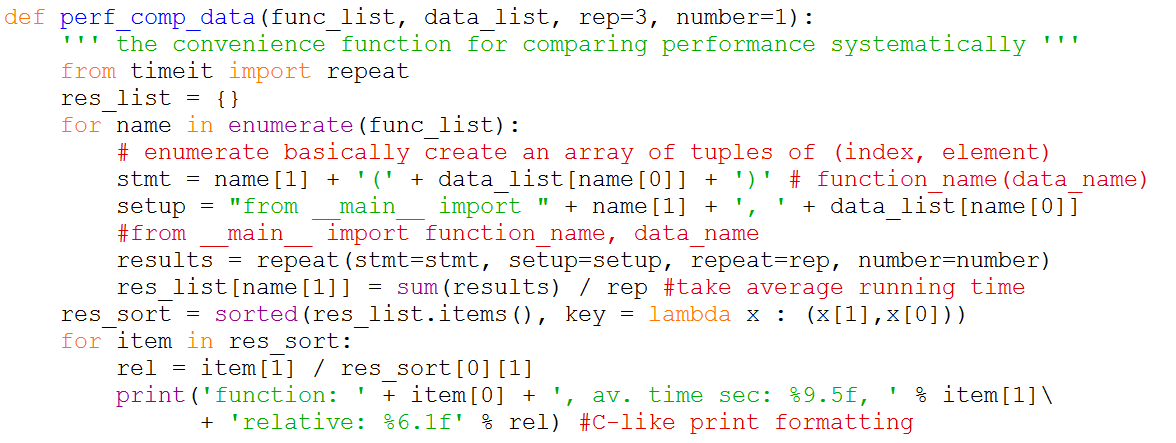
\includegraphics[scale=0.4]{convenience_function.png}
\end{figure}
\end{frame}

\subsection{Improvements in execution speed}

\begin{frame}
\frametitle{Numerical operations}
Multithreaded numexpr implementation is fastest compared to:\\[3mm]
\begin{itemize}
	\item using \emph{eval} function
	\item using built-in library math
	\item using iterators (lists)
	\item using numpy's mathematical methods
	\item using single-threaded numexpr
\end{itemize}
\begin{figure}[H]
	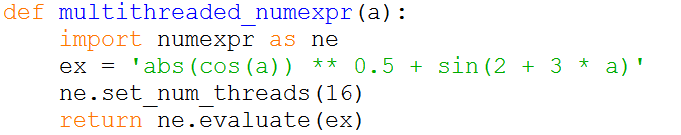
\includegraphics[scale=0.6]{multithreaded_numexpr.png}
\end{figure}
\end{frame}
%------------------------------------------------

\begin{frame}
\frametitle{Highly computational burden problems}
Parallel calculations are superior in heavy workloads\\
There are two different ways to conduct parallel calculations
\begin{itemize}
	\item IPython.parallel (or ipyparallel) using cluster
	\item using the standard library multiprocessing
	\item massive parallel operations using GPGPUs
\end{itemize}
Multiprocessing is a standard built-in library, hence recommended
\begin{figure}[H]
	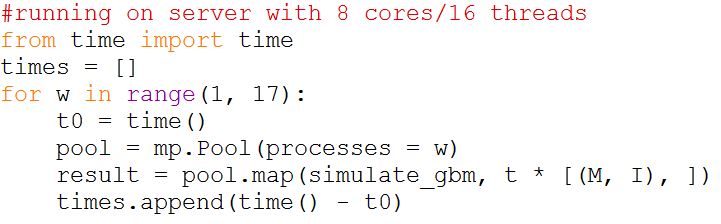
\includegraphics[scale=0.6]{multiprocessing.png}
\end{figure}
\end{frame}
%------------------------------------------------


%------------------------------------------------
\subsection{Preserving memory efficiency}

%------------------------------------------------
\begin{frame}
\frametitle{Compiling to improve memory efficiency}
NumPy is significantly faster than normal python\\
but it is using 8 times of memory compared to normal python!\\
There are two other ways to resolve this with the same computation speed
\begin{itemize}
	\item Dynamic compiling using numba
	\item Static compiling using Cython
\end{itemize}
Cython preserves the same speed with numba in dealing with nested loops\\
numba has another advantage introduced in the next page!
\end{frame}

%------------------------------------------------
\subsection{Efficiency in writing code}

\begin{frame}
\frametitle{Little additional effort to improve performance}
\begin{itemize}
	\item numpy requries us to think of the matrix form
	\item numba only requires to call the \textbf{jit} function
	\item numba also preserve the memory efficiency
	\item numba seems to be the best choice!
\end{itemize}
\begin{figure}[H]
	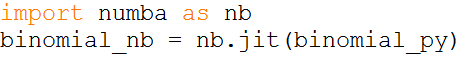
\includegraphics[scale=0.8]{numba_jit.png}
\end{figure}
\end{frame}

%------------------------------------------------
\begin{frame}
\frametitle{Code sample for binomial option pricing}
\begin{figure}[H]
	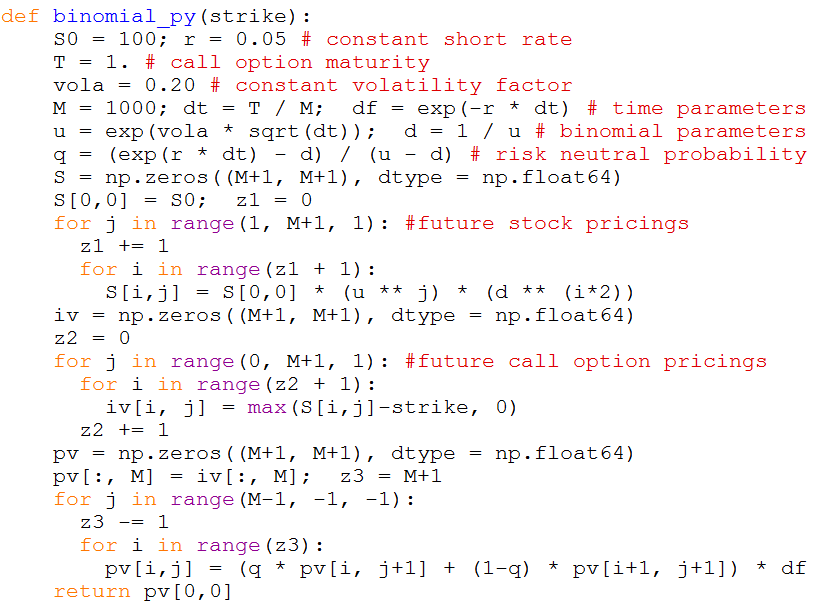
\includegraphics[scale=0.48]{binomial_option_pricing.png}
\end{figure}
\end{frame}

%------------------------------------------------
\section{Stochastics}
%------------------------------------------------
\begin{frame}
\frametitle{Chapter 10 Stochastics}
\begin{itemize}
	\item Random number geneartion
	\item Simulation
	\item Valuation
	\item Risk measures
\end{itemize}
\end{frame}

%------------------------------------------------
\subsection{Random number generation}
\begin{frame}
\frametitle{Random number generation}
using functions provided in \emph{numpy.random}\\
(import numpy.random as npr: for convenience)
\begin{itemize}
	\item Standard normal: npr.standard\_normal(sample\_size)
	\item Normal: npr.normal(mu, sigma, sample\_size)
	\item Chi Square: npr.chisquare(df = 0.5, size = sample\_size)
	\item Poisson: npr.poisson(lam = 1.0, size = sample\_size)
\end{itemize}
The return value of the above methods are numpy arrays
\end{frame}

%------------------------------------------------
\subsection{Simulation}
\begin{frame}
\frametitle{Simulation}
\begin{itemize}
	\item Geometric Brownian Motion
	\item Square-root Diffusion Model
	\item Jump Diffusion Model
	\item Stochastic Volatility Model
\end{itemize}
\end{frame}

\begin{frame}
\frametitle{Simulation for Geometric Brownian Motion}
\begin{center}
We have two different ways to generate simulations for this equation:\\
$$S_{T} = S_{0}\exp\{(r-\frac{1}{2}\sigma^{2})T + \sigma\sqrt{T}z\}$$
\end{center}
\begin{figure}[H]
	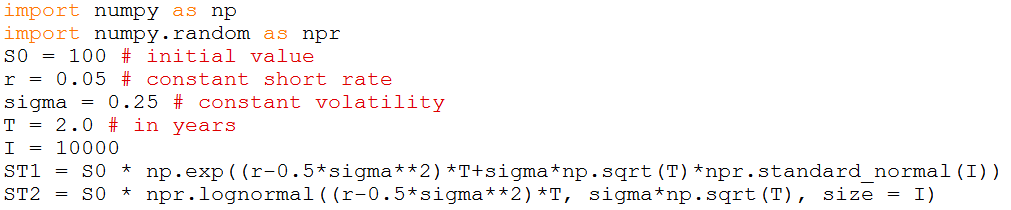
\includegraphics[scale=0.45]{simulate_GBM_T.png}
\end{figure}
\end{frame}

%------------------------------------------------
\begin{frame}
\frametitle{Simulation for Geometric Brownian Motion}
\begin{center}
$S_{t} = S_{t-^{\Delta}t}\exp\{(r-\frac{1}{2}\sigma^{2})^{\Delta}t + \sigma\sqrt{^{\Delta}t}z_{t}\}$
\end{center}
\begin{figure}[H]
	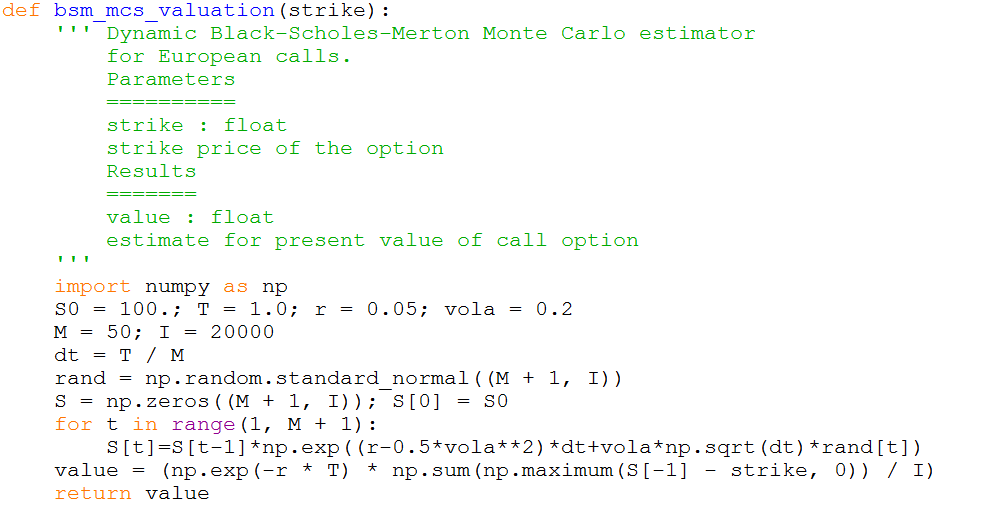
\includegraphics[scale=0.45]{mcs_gbm.png}
\end{figure}
\end{frame}

%------------------------------------------------
\begin{frame}
\frametitle{Simulation for Stochastic volatility model}
\begin{center}
	$dS_{t} = rS_{t}dt + \sqrt{v_{t}}S_{t}dZ_{t}^{1}$\\[3mm]
	$dv_{t} = \kappa_{v}(\theta_{v}-v_{t})dt + \sigma_{v}\sqrt{v_{t}}dZ_{t}^{2}$\\[3mm]
	$dZ_{t}^{1}dZ_{t}^{2} = \rho $
\end{center}
\emph{Euler discretization}:
\begin{center}
	$v_{t} = v_{t-^{\Delta}t} + \kappa(\theta-v_{t-^{\Delta}t}){^{\Delta}t} + \sigma\sqrt{^{\Delta}t*v_{t-^{\Delta}t}}z_{t}^{2}$\\[3mm]
	$S_{t} = S_{t-^{\Delta}t} \exp\{(r-\frac{1}{2}v_{t}){^{\Delta}t}+\sqrt{v_{t}{^{\Delta}t}}z_{t}^{1}\}$
\end{center}
Still we need to ensure that:
\begin{center}
	$dZ_{t}^{1}dZ_{t}^{2} = \rho $
\end{center}
\end{frame}

%------------------------------------------------
\begin{frame}
\frametitle{Simulation for Stochastic volatility model}
\begin{center}
	$v_{t} = v_{t-^{\Delta}t} + \kappa(\theta-v_{t-^{\Delta}t}){^{\Delta}t} + \sigma\sqrt{^{\Delta}t*v_{t-^{\Delta}t}}z_{t}^{2}$
	$S_{t} = S_{t-^{\Delta}t} \exp\{(r-\frac{1}{2}v_{t}){^{\Delta}t}+\sqrt{v_{t}{^{\Delta}t}}z_{t}^{1}\}$
\end{center}
\begin{figure}[H]
	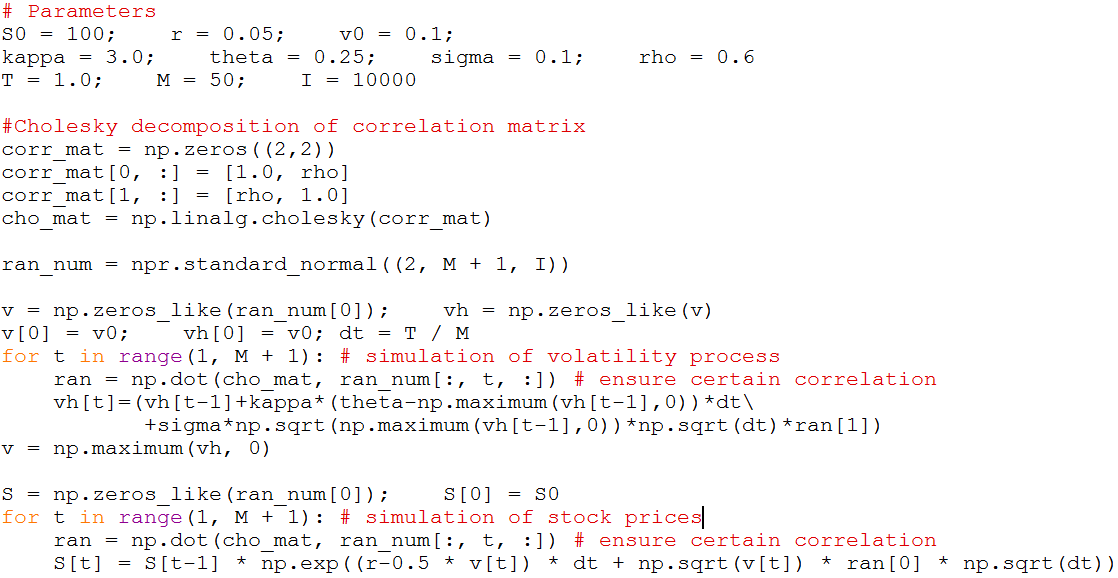
\includegraphics[scale=0.4]{stochastic_volatility.png}
\end{figure}
\end{frame}

%------------------------------------------------
\begin{frame}
\frametitle{Simulation for Square-root diffusion model}
\begin{center}
	$dx_{t} = \kappa(\theta-x_{t})dt + \sigma\sqrt{x_{t}}dZ_{t}$
\end{center}
\emph{Euler discretization}:
\begin{center}
	letting $s = t-^{\Delta}t$, and $x^{+} = max(x,0)$\\[3mm]
	$\tilde{x}_{t} = \tilde{x}_{s} + \kappa(\theta-\tilde{x}_{s}^{+}){^{\Delta}t} + \sigma\sqrt{\tilde{x}_{s}^{+}{^{\Delta}t}}z_{t}$\\[3mm]
	$x_{t} = \tilde{x}_{t}^{+}$
\end{center}
\end{frame}

%------------------------------------------------
\begin{frame}
\frametitle{Simulation for Square-root diffusion model}
With the Euler discretization:
\begin{center}
	letting $s = t-^{\Delta}t$, and $x^{+} = max(x,0)$\\[3mm]
	$\tilde{x}_{t} = \tilde{x}_{s} + \kappa(\theta-\tilde{x}_{s}^{+}){^{\Delta}t} + \sigma\sqrt{\tilde{x}_{s}^{+}{^{\Delta}t}}z_{t}$\\[3mm]
	$x_{t} = \tilde{x}_{t}^{+}$
\end{center}
\begin{figure}[H]
	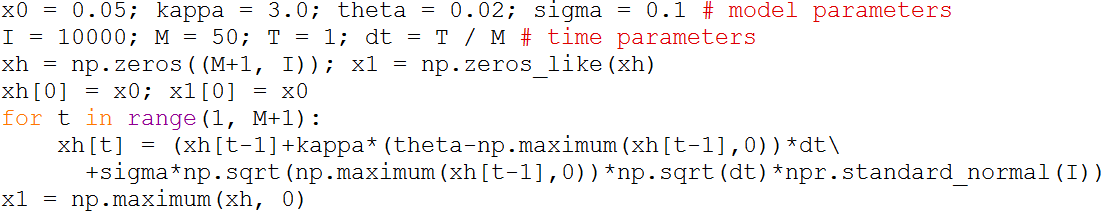
\includegraphics[scale=0.4]{square_root_diffusion.png}
\end{figure}
\end{frame}

%------------------------------------------------
\begin{frame}
\frametitle{Simulation for Square-root diffusion model}
With the exact Euler discretization:
\begin{center}
	letting $s = t-{^{\Delta}t}$\\[3mm]
	$x_{t} = \frac{\sigma^{2}(1-e^{-\kappa{^{\Delta}t}})}{4\kappa}\chi_{d}^{2}[\frac{4\kappa e^{-\kappa{^{\Delta}t}}}{\sigma^{2}(1-e^{-\kappa{^{\Delta}t}})}x_{s}]$
\end{center}
\begin{figure}[H]
	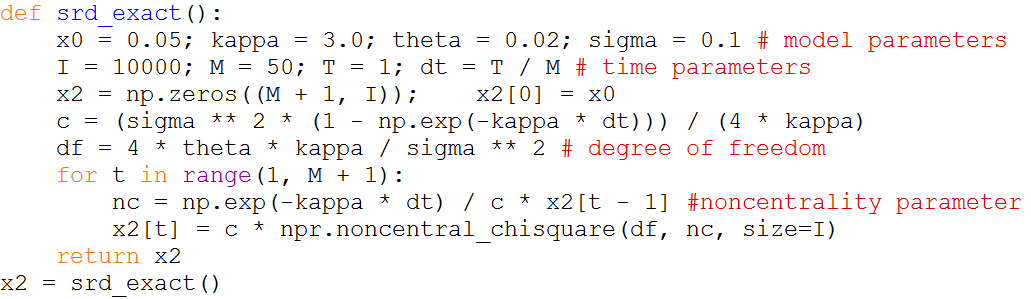
\includegraphics[scale=0.4]{square_root_diffusion_exact.png}
\end{figure}
\end{frame}

%------------------------------------------------
\begin{frame}
\frametitle{Simulation for jump diffusion model}
\begin{center}
	$dS_{t} = (r-r_{\mathrm{J}})S_{t}dt + S_{t}dZ_{t}	+ {\mathrm{J}}_{t}S_{t}dN_{t}$\\[10mm]
	Euler discretization:\\[6mm]
	$S_{t} = S_{t-{^{\Delta}t}} [e^{(r-r_{\mathrm{J}}-\sigma^{2}/2){^{\Delta}t}+\sigma \sqrt{^{\Delta}t}z_{t}^{1}}+(e^{\mu_{\mathrm{J}}+\delta z_{t}^{2}}-1)y_{t}] $
\end{center}
\end{frame}

%------------------------------------------------
\begin{frame}
\frametitle{Simulation for jump diffusion model}
\begin{center}
	Euler discretization:\\[3mm]
	$S_{t} = S_{t-{^{\Delta}t}} [e^{(r-r_{\mathrm{J}}-\sigma^{2}){^{\Delta}t}+\sigma \sqrt{^{\Delta}t}z_{t}^{1}}+(e^{\mu_{\mathrm{J}}+\delta z_{t}^{2}}-1)y_{t}] $
\end{center}
\begin{figure}[H]
	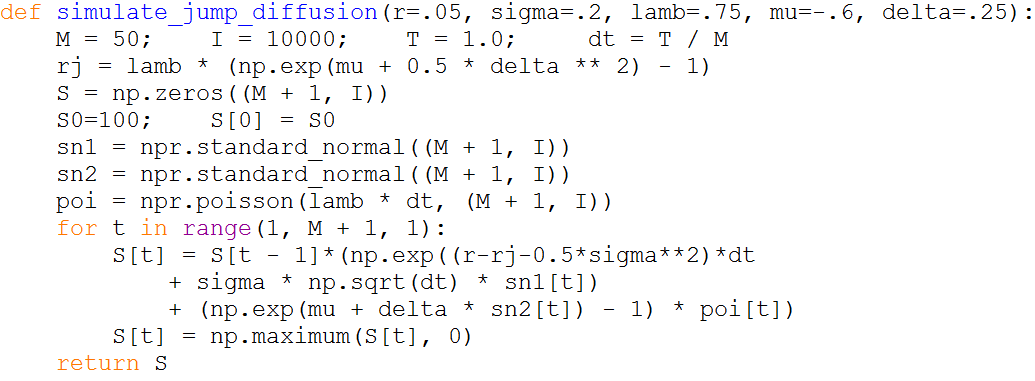
\includegraphics[scale=0.44]{simulate_jump_diffusion.png}
\end{figure}
\end{frame}

%------------------------------------------------
\begin{frame}
\frametitle{Variance Reduction}
There are two main techniques
\begin{itemize}
	\item antithetic variates - first moment
	\item moment matching - first and second moments
\end{itemize}
\begin{figure}[H]
	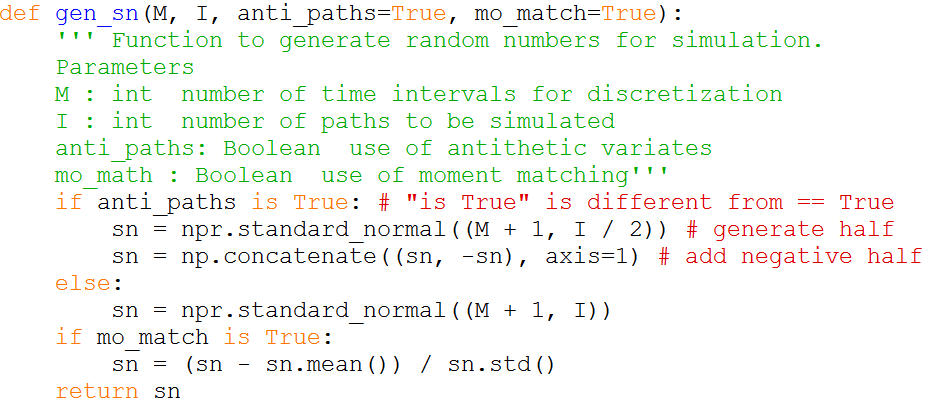
\includegraphics[scale=0.5]{variance_reduction.png}
\end{figure}
\end{frame}

\subsection{Valuation}
%------------------------------------------------
\begin{frame}
\frametitle{Valuation}
We will be doing valuation on two different types of derivatives\\ [4mm]
\begin{itemize}
	\item European options\\[9mm]
	\item American options
\end{itemize}
\end{frame}

%------------------------------------------------
\begin{frame}
\frametitle{Valuation - European options}
\begin{center}
European options\\ [8mm]
Pricing by risk-neutral expectation\\ [3mm]
$C_{0} = e^{-rT} \mathbb{E}_{0}^{Q}(h(S_{T})) = e^{-rT} \int_{0}^{\infty} h(s)q(s) \,ds $\\ [6mm]
Risk-neutral Monte Carlo estimator
$$\tilde{C}_{0} = e^{-rT} \frac{1}{\mathrm{I}} \sum_{i=1}^{\mathrm{I}} h({\tilde{S}}_{T}^{i}) $$
\end{center}
\begin{flushright}
where $h(S_{t})$ stands for the payoff function, \\
$S_{t}$ is the index level at maturity, \\
and $\tilde{S}_{t}^{i} $ stands for the ith simulated index level at maturity
\end{flushright}
\end{frame}

%------------------------------------------------
\begin{frame}
\frametitle{Valuation - European call options}
\begin{center}
$$\tilde{C}_{0} = e^{-rT} \frac{1}{\mathrm{I}} \sum_{i=1}^{\mathrm{I}} h({\tilde{S}}_{T}^{i}) $$
$\tilde{S}_{T} = S_{0}\exp\{(r-\frac{1}{2}\sigma^{2})T + \sigma\sqrt{T}\tilde{z}_{T}\}$\\[5mm]
\begin{figure}[H]
	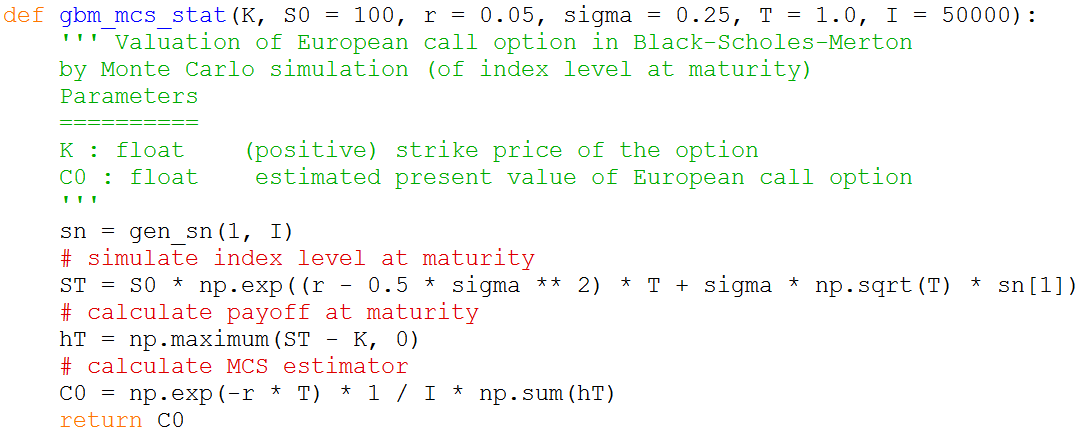
\includegraphics[scale=0.4]{european_call_mcs.png}
\end{figure}
\end{center}
\end{frame}

%------------------------------------------------
\begin{frame}
\frametitle{Valuation - European options}
\begin{center}
We can make a generic pricing function!
$$\tilde{C}_{0} = e^{-rT} \frac{1}{\mathrm{I}} \sum_{i=1}^{\mathrm{I}} h({\tilde{S}}_{T}^{i}) $$
$\tilde{S}_{T} = S_{0}\exp\{(r-\frac{1}{2}\sigma^{2})T + \sigma\sqrt{T}\tilde{z}_{T}\}$
\begin{figure}[H]
	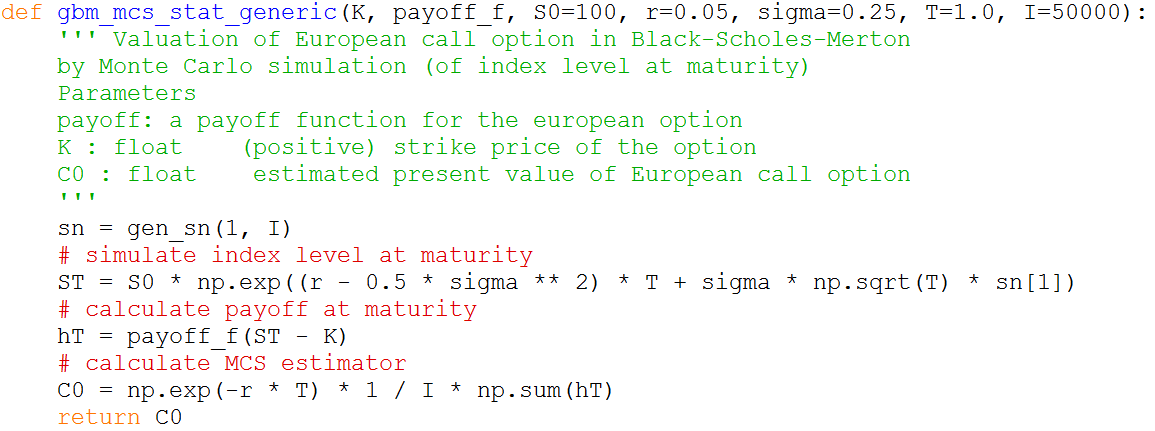
\includegraphics[scale=0.4]{european_option_mcs.png}
\end{figure}
\end{center}
\end{frame}

%------------------------------------------------
\begin{frame}
\frametitle{Valuation - European options}
\begin{center}
Testing the generic pricing function using payoff function of call option\\[3mm]
\begin{figure}[H]
	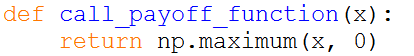
\includegraphics[scale=0.8]{call_payoff_function.png}
\end{figure}
\begin{figure}[H]
	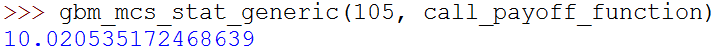
\includegraphics[scale=0.6]{test_european_option_mcs.png}
\end{figure}
\begin{figure}[H]
	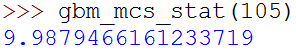
\includegraphics[scale=0.6]{test_european_call_mcs.png}
\end{figure}
\end{center}
\end{frame}

%------------------------------------------------
\begin{frame}
\frametitle{Valuation - European options}
\begin{center}
We can adopt the dynamic simulation approach
\begin{figure}[H]
	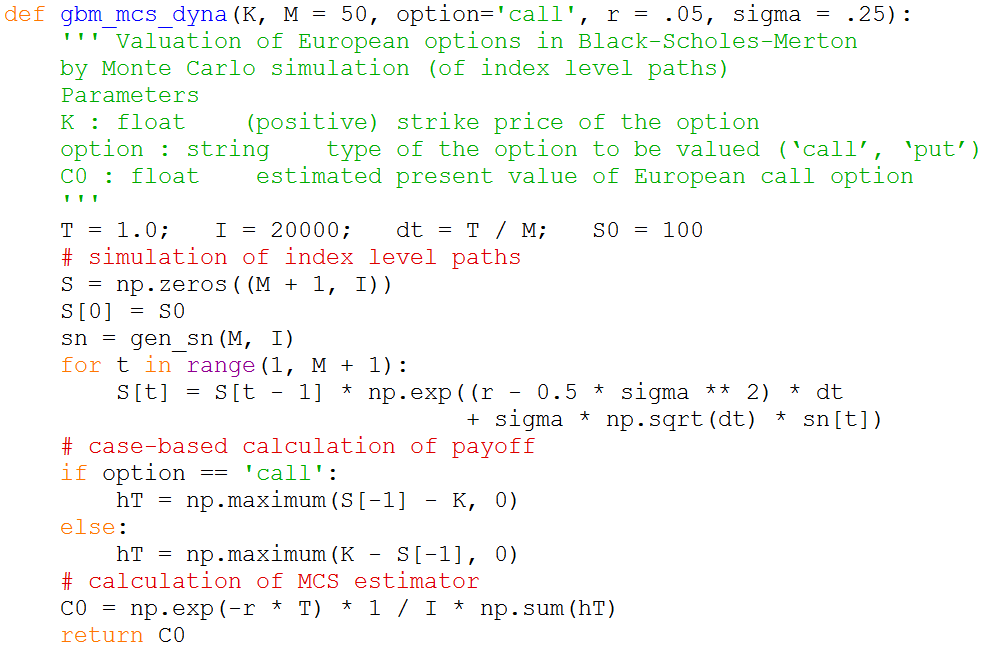
\includegraphics[scale=0.41]{european_option_mcs_dynamic.png}
\end{figure}
\end{center}
\end{frame}

%------------------------------------------------
\begin{frame}
\frametitle{Valuation - American options}
\begin{center}
optimal stopping approach - theory not understood yet
$$V_{0} = \sup_{\tau \in \{ 0, {^{\Delta}t}, 2{^{\Delta}t}, \dots, T \}} e^{-rT} \mathbb{E}_{0}^{Q}(h_{\tau}(S_{\tau}))$$
Least-sqaures regression for American option valuation
$$ \min_{\alpha_{1,t}, \dots, \alpha_{D,t}} \frac{1}{\mathrm{I}} \sum_{d=1}^{D} (\alpha_{d,t}\cdot b_{d}(S_{t}, i))^{2} $$
\end{center}
\end{frame}

%------------------------------------------------
\begin{frame}
\frametitle{Valuation - American options}
\begin{figure}[H]
	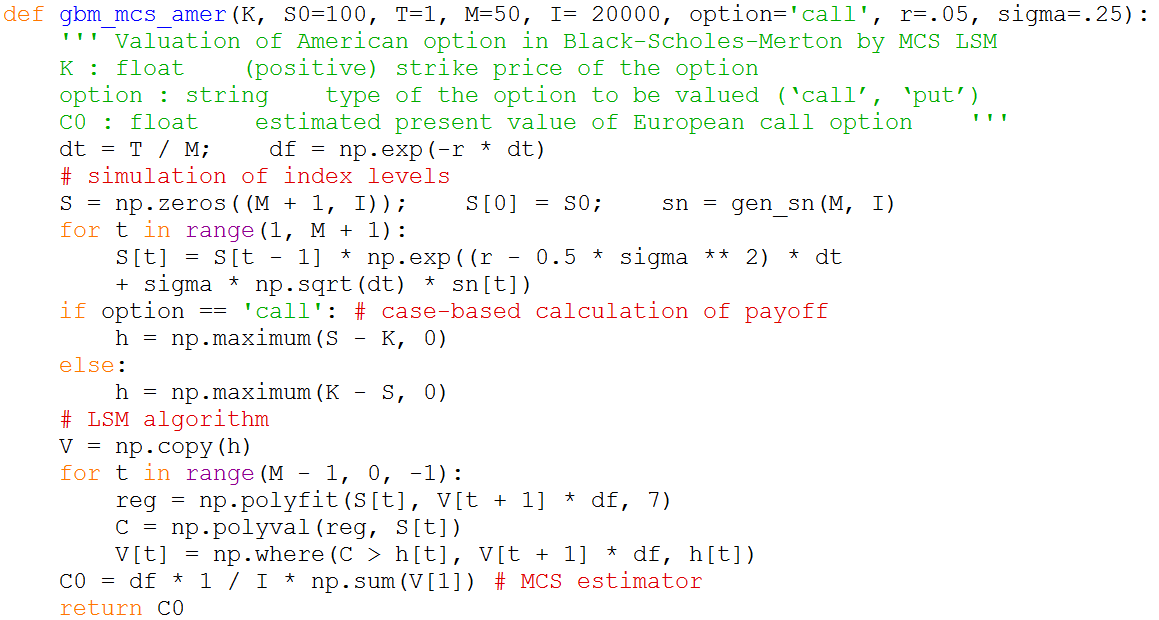
\includegraphics[scale=0.4]{gbm_mcs_amer.png}
\end{figure}
\end{frame}

%------------------------------------------------
\subsection{Risk measures}
%------------------------------------------------
\begin{frame}
\frametitle{Risk measures}
\begin{itemize}
	\item Value at Risk
	\item Credit Value Adjustment
\end{itemize}
\end{frame}

%------------------------------------------------
\begin{frame}
\frametitle{Value at Risk - Black Scholes' World}
\begin{center}
Holding a stock has probability of $x$\% to suffer a loss greater than $y$\\[3mm]
scs: scipy.stats
\end{center}
\begin{figure}[H]
	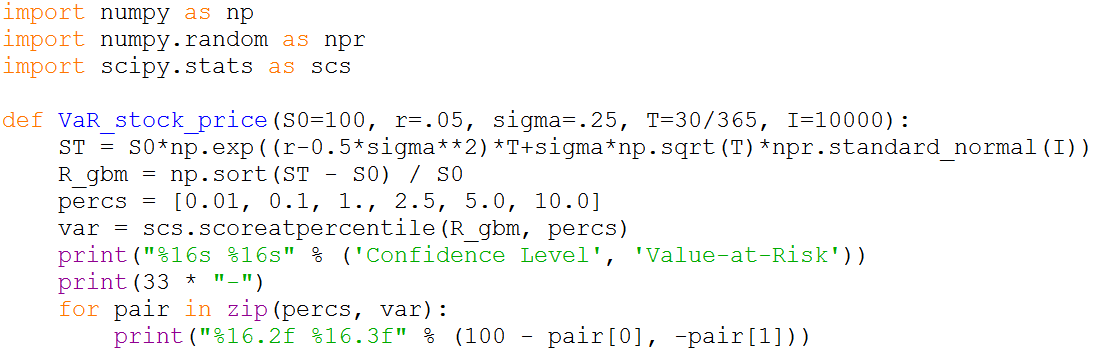
\includegraphics[scale=0.42]{VaR_stock_price.png}
\end{figure}
\end{frame}

%------------------------------------------------
\begin{frame}
\frametitle{Value at Risk - Jump Diffusion Model}
\begin{center}
Holding a stock has probability of $x$\% to suffer a loss greater than $y$
\end{center}
\begin{figure}[H]
	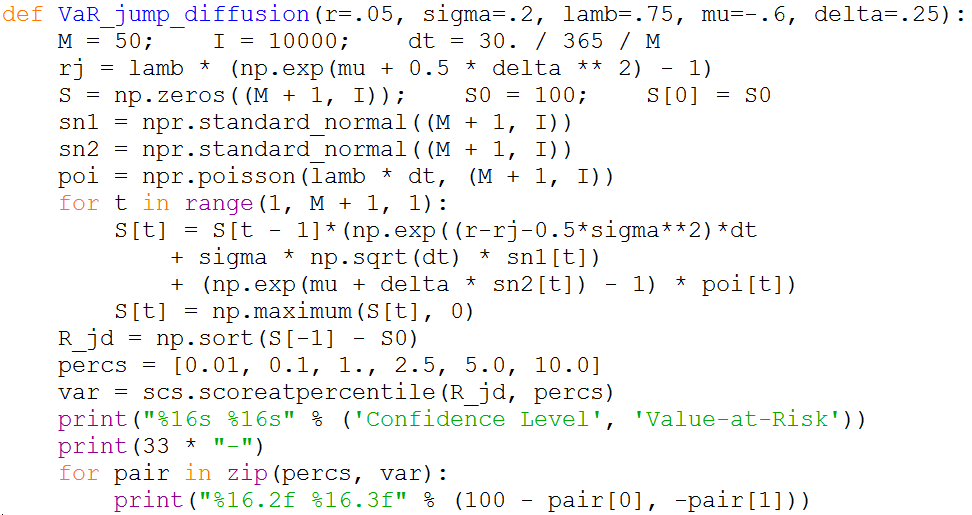
\includegraphics[scale=0.42]{VaR_jump_diffusion.png}
\end{figure}
\end{frame}

%------------------------------------------------
\begin{frame}
\frametitle{Credit Value Adjustment through CVaR}
\begin{center}
Holding a stock has probability of $x$\% to suffer a loss greater than $y$
\end{center}
\begin{figure}[H]
	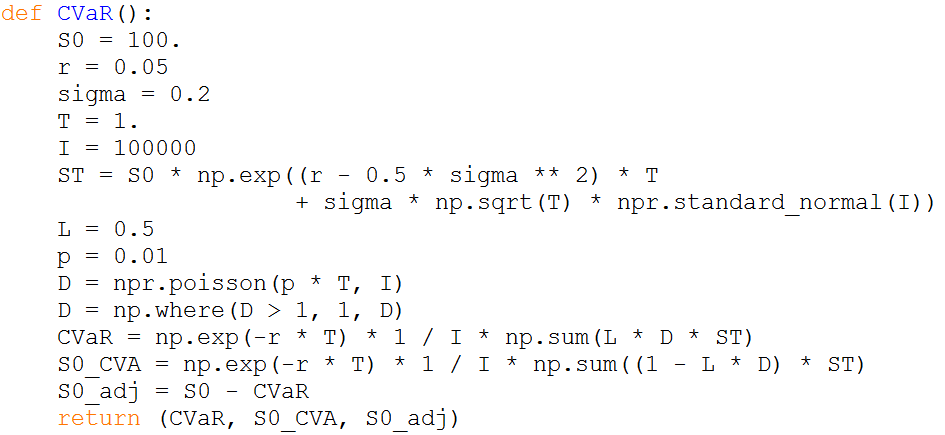
\includegraphics[scale=0.45]{CVaR.png}
\end{figure}
\end{frame}

%------------------------------------------------
\begin{frame}
\Huge{\centerline{Thank You}}
\begin{center}
\begin{normalsize}
\emph{E0007424@u.nus.edu}
\end{normalsize}
\end{center}
\end{frame}


%------------------------------------------------

\end{document} 